%%%%%%%%%%%%%%%%%%%%%%%%%%%%%%%%%%%%%%%%%%%%%%%%%%%%%%%%%%%%%%%%%
\subsection{Analyse}	%	RMINIMUM - Analyse
%%%%%%%%%%%%%%%%%%%%%%%%%%%%%%%%%%%%%%%%%%%%%%%%%%%%%%%%%%%%%%%%%


\noindent
In diesem Abschnitt werden der Algorithmus \Rm im Gesamten und seine einzelnen Phasen theoretisch analysiert.\\
Hierbei ist die Auswahl der diskutierten Bereiche und Theoreme auf die für diese Arbeit relevanten Aussagen eingeschränkt. Für weitere Informationen sei hier auf das Paper~\cite{meyer1} verwiesen.\\[.1cm]
\noindent\makebox[\linewidth]{\color{gray}{\hdashrule[0.5ex]{\linewidth}{0.5pt}{1.5mm}}}\\[.05cm]
% ---------------------------------------------------------------
%	Phase 1
\noindent
\begin{minipage}[Ht]{.44\textwidth}
\textbf{Phase 1.} In der ersten Phase nimmt jedes der $n$ Elemente an genau einem Vergleich teil. Da je zwei Elemente an einem Vergleich teilnehmen, folgt insgesamt:\\

\noindent
$\mfge = 1$, $\forall e\in X$ und somit\\[.05cm]
$\mfgm = \mfgr = \mfgc = 1$ sowie\\[.05cm]
$w(n)=n/2$ für die verrichtete Arbeit.\\[.05cm]
\end{minipage}% This must go next to `\end{minipage}`
%
\hfill
%
\begin{minipage}[Ht]{.54\textwidth}
        \centering
        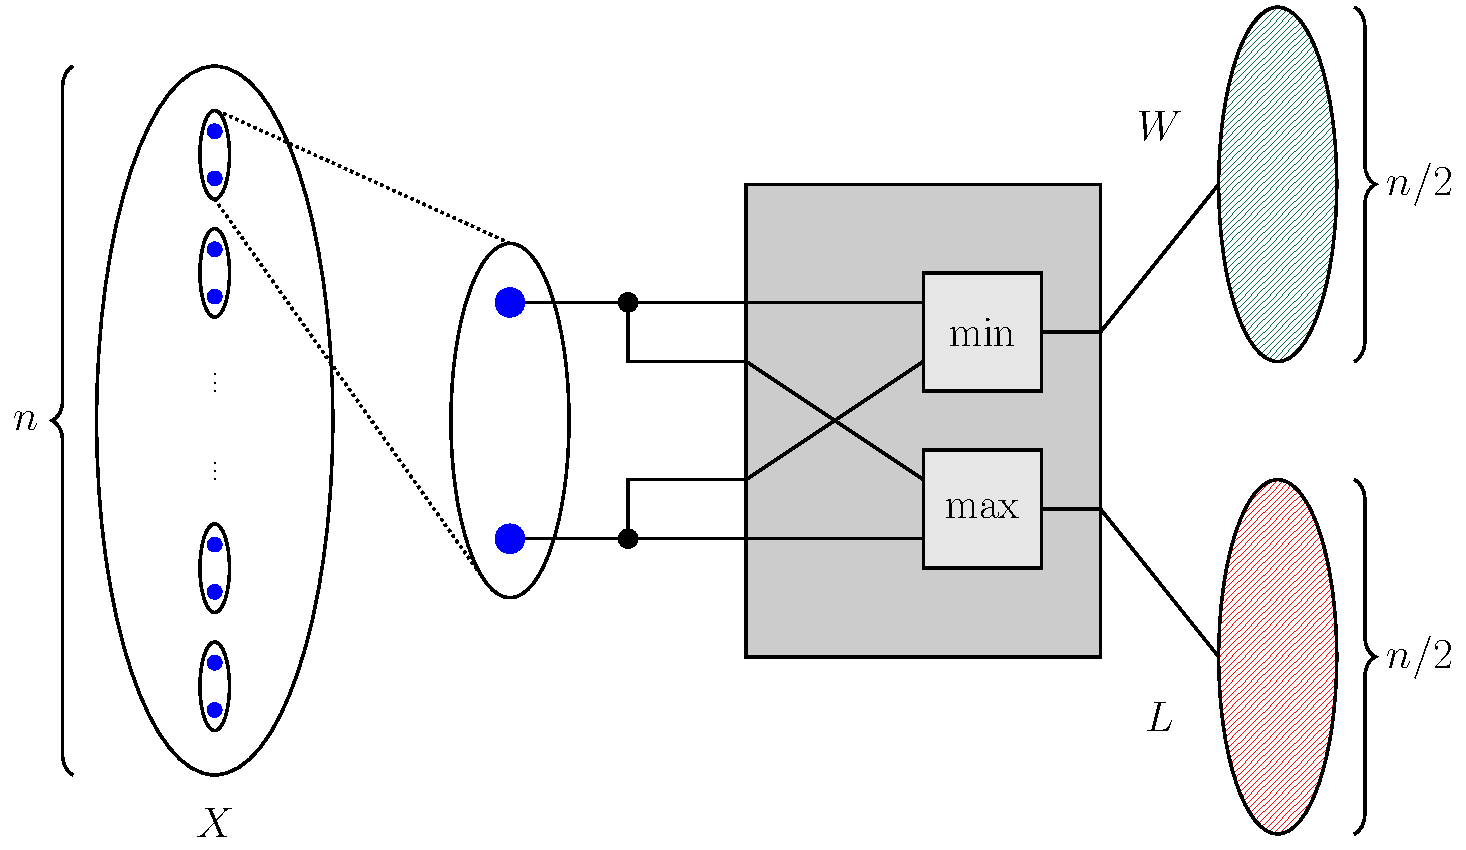
\includegraphics[scale=0.35]{snippets/tikz/min_p1.pdf}
        \vspace*{-4mm}
        \captionof{figure}{Visualisierung Phase 1}\label{fig: min_p1}
        %
        \vspace*{0.1cm}
\end{minipage}

\noindent\makebox[\linewidth]{\color{gray}{\hdashrule[0.5ex]{\linewidth}{0.5pt}{1.5mm}}}\\[.05cm]
% ---------------------------------------------------------------
%	Phase 2
\noindent
\begin{minipage}[Ht]{.34\textwidth}
\textbf{Phase 2.} In der zweiten Phase gilt aufgrund des ausbalancierten Turnierbaums $1 \leq f_{x_l}(n)\leq \log_2(k)$ $\forall x_l\in L$ und $f_{x_w}(n)=0$ $\forall x_w\in W$ sowie Insbesondere $\mfgm = 0$ und $\mfgr = \log_2(k)$.\\[.15cm]
\end{minipage}% This must go next to `\end{minipage}`
%
\hfill
%
\begin{minipage}[Ht]{.64\textwidth}
        \centering
        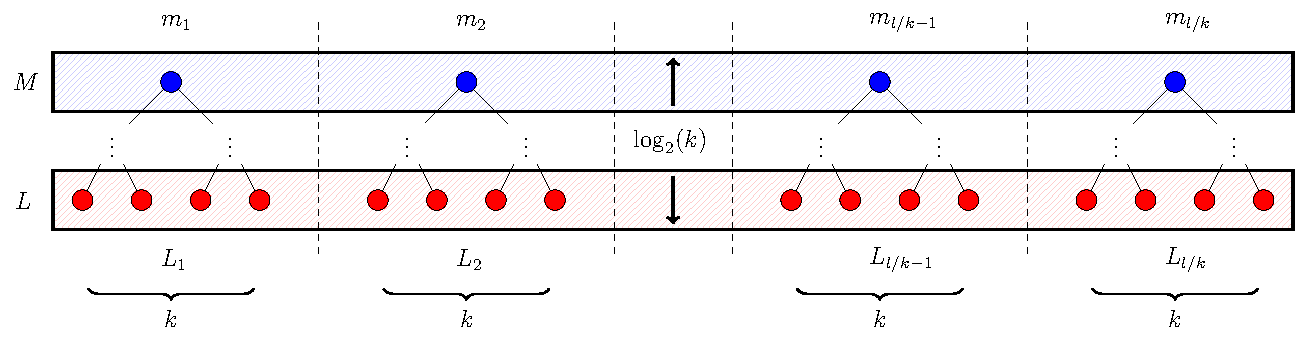
\includegraphics[scale=0.5]{snippets/tikz/min_p2.pdf}
        \vspace*{-10mm}
        \captionof{figure}{Visualisierung Phase 2}\label{fig: min_p1}
\end{minipage}
%
\noindent
Um in einem perfekt ausbalancierten Turnierbaum bei $k$ Teilnehmern einen Sieger zu ermitteln, bedarf es $k-1$ Vergleiche. Da es $n/2k$ Teilmengen gibt, ergibt sich $w(n)\leq (k-1)\cdot (n/2k) = n/2 - n/2k = \mO(n)$.\\[.05cm]
\noindent\makebox[\linewidth]{\color{gray}{\hdashrule[0.5ex]{\linewidth}{0.5pt}{1.5mm}}}\\[.05cm]
% ---------------------------------------------------------------
%	Phase 3
\noindent
\textbf{Phase 3.} In der dritten Phase wird jedes Element aus $W$ genau ein mal mit einem Element $m_i$ verglichen. Es gilt somit $f_{x_w}(n)=1$ $\forall x_w\in W$ sowie $f_{m_i}(n)\leq k$ $\forall m_i$.\\
Für die in Phase 3 verrichtete Arbeit gilt $w(n)\leq n/2 + k\cdot n/2=\mO(n)$.\\[.05cm]
\noindent\makebox[\linewidth]{\color{gray}{\hdashrule[0.5ex]{\linewidth}{0.5pt}{1.5mm}}}\\[.05cm]
% ---------------------------------------------------------------
%	Phase 4
\noindent
\textbf{Phase 4.} Die vierte Phase unterscheidet zwei Fälle. Wird die angegebene Schranke eingehalten, so gilt $1\leq f_{x_{w'}}(n)\leq \log_2(|W'|)$ $\forall x_{w'}\in W'$ sowie $f_e(n)=0$ $\forall e\notin W'$.\\
Insbesondere gilt $\mfgm = \log_2(|W'|)$ sowie $\mfgr = \log_2(|W'|)-1$.\\[.075cm]
In diesem Fall gilt für die verrichtete Arbeit $w(n)=|W'|-1=\mO(n)$.\\[.075cm]
Im zweiten Fall findet ein rekursiver Aufruf statt, sodass keinerlei Vergleiche stattfinden.
\\[.05cm]
\noindent\makebox[\linewidth]{\color{gray}{\hdashrule[0.5ex]{\linewidth}{0.5pt}{1.5mm}}}\\[.05cm]
% ---------------------------------------------------------------
%	Algo
\noindent
\textbf{RMinimum.} Für den gesamten Algorithmus ist relevant festzustellen, dass die Wahrscheinlichkeit, die Schranke der vierten Phase einzuhalten, von der Randomisierung der vorherigen Phasen abhängig ist. Dementsprechend ist die Mächtigkeit der Menge $|W'|$ bei wiederholter Ausführung mit gleicher Parametrisierung immer noch zufällig, wobei die stochastische Verteilung abhängig von der Wahl der Parameter ist.\\[.2cm]
Folgende Aussagen wollen wir im Laufe dieser Arbeit experimentell unterstützen.\\[.05cm]
\noindent\makebox[\linewidth]{\color{gray}{\hdashrule[0.5ex]{\linewidth}{0.5pt}{1.5mm}}}
% ---------------------------------------------------------------
%	Theoreme
%================================================================
\begin{manualtheorem}{3}\label{theo: min_3}
\Rm benötigt lineare Arbeit, also $w(n)=\mO(n)$.
\end{manualtheorem}
\begin{proof}
Betrachte einen beliebigen Rekursionsschritt mit einer Eingabemenge der Mächtigkeit $n'$. Die erste Phase benötigt $\mO(n')$ viele Vergleiche um die Mengen $W$ und $L$ zu bestimmen. Des Weiteren beinhaltet die Menge $W'$ kein Element der Menge $L$ und es folgt $w(n)= w(|W'|) + \mO(n) \leq w(n/2) + \mO(n) = \mO(n)$. 
\end{proof}
%================================================================
\begin{manuallemma}{2}\label{lem: min_2}
Sei $W_i$ eine beliebige Siegerpartition sowie $m_i$ das zum Filtern genutzte Minimum und $W'_i=\{w|w\in W_i \wedge w_i < m_i\}$ die Menge aller Elemente, die kleiner als $m_i$ sind.\\
Dann gilt $\mathbb{E}[|W'_i|]\leq 2d\sqrt{k}$ für eine Konstante $d>0$.
\end{manuallemma}
%================================================================
\begin{manualtheorem}{4}\label{theo: min_4}
Sei $k(n)=n^{\varepsilon}$ für $0<\varepsilon<1/2$. Dann benötigt \Rm $\mathbb{E}[f_{min}]=\mathcal{O}(\varepsilon^{-1}\log\log(n))$ Vergleiche für das \mE und $\mathbb{E}[f_{rem}]=\mathbb{O}(n^{\varepsilon})$ für alle übrigen Elemente.
\end{manualtheorem}
%================================================================
\begin{manualtheorem}{5}\label{theo: min_5}
Sei $k(n)=\log(n)/\log\log(n)$. Dann benötigt \Rm $\mathbb{E}[f_{min}]=\mathcal{O}(\log(n)/\log\log(n))$ Vergleiche für das \mE und $\mathbb{E}[f_{rem}]=\mathcal{O}(\log(n)/\log\log(n))$ für alle übrigen Elemente.
\end{manualtheorem}

\noindent\makebox[\linewidth]{\color{gray}{\hdashrule[0.5ex]{\linewidth}{0.5pt}{1.5mm}}}\\[.05cm]
% ---------------------------------------------------------------
%	Ende
\noindent
Die aufgeführten Theoreme und Lemmata dienen als Grundlage für den Analyseschwerpunkt und somit auch für die in dieser Arbeit zugrunde liegende Implementierung. 











